\documentclass[tikz,border=5mm,12pt]{standalone}
\usepackage[fontsize=16pt]{fontsize}

\begin{document}
  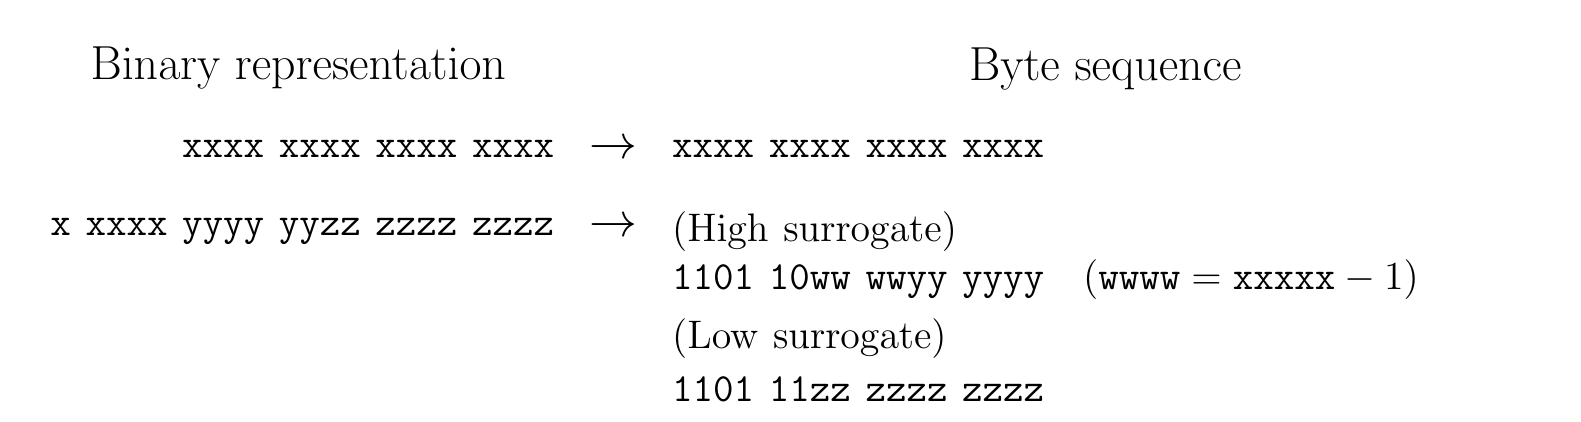
\begin{tikzpicture}
    \node[text width=65mm,align=center] at (0,0) {Binary representation\strut};
    \node[text width=65mm,align=right] at (0,-10mm) {\small\texttt{xxxx xxxx xxxx xxxx}\strut};
    \node[text width=65mm,align=right] at (0,-20mm) {\small\texttt{x xxxx yyyy yyzz zzzz zzzz}\strut};

    \node at (40mm,-10mm) {$\rightarrow$\strut};
    \node at (40mm,-20mm) {$\rightarrow$\strut};

    \node[text width=110mm,align=center] at (102.5mm,0) {Byte sequence};
    \node[text width=110mm,align=left] at (102.5mm,-10mm) {\small\texttt{xxxx xxxx xxxx xxxx}\strut};
    \node[text width=110mm,align=left,text depth=0mm,minimum height=42.5mm] at (102.5mm,-20mm) {\small (High surrogate)\\
      \texttt{1101 10ww wwyy yyyy}\strut \quad$(\texttt{wwww} = \texttt{xxxxx}-1)$\\
      \vspace{4pt}
      (Low surrogate) \\
      \texttt{1101 11zz zzzz zzzz}\strut};
  \end{tikzpicture}
\end{document}
